\RequirePackage{fix-cm}
\documentclass[smallextended,natbib]{../template/svjour3}

\smartqed

\usepackage[T1]{fontenc}
\usepackage[utf8]{inputenc}
\usepackage{graphicx}
\usepackage{float}
\usepackage{longtable}
\usepackage{listings}
\usepackage{makecell}
\usepackage{amsmath}
\usepackage{siunitx}
\usepackage[hidelinks]{hyperref}

\hypersetup{
  pdftitle={LLM-Based SQL Antipattern Detection in jOOQ Code: An Occurrence-Level Evaluation and Repository Study},
  pdfauthor={Kristo Isberg; Erki Eessaar},
  pdfsubject={Manuscript for Empirical Software Engineering},
  pdfkeywords={SQL antipatterns, jOOQ, large language models, static analysis, prompting, empirical software engineering}
}

\journalname{Empirical Software Engineering}

\newcommand{\sotaModel}{OpenAI GPT-5.2 (reasoning)}
\newcommand{\sotaModelNl}{OpenAI GPT-5.2\\(reasoning)}
\newcommand{\openModel}{Z.ai GLM-5 (reasoning)}
\newcommand{\openModelNl}{Z.ai GLM-5 (reasoning)}
\newcommand{\nonReasoningModel}{Anthropic Claude Opus 4.5 (non-reasoning)}
\newcommand{\nonReasoningModelNl}{Anthropic Claude Opus\\4.5 (non-reasoning)}
\newcommand{\mediumModel}{OpenAI gpt-oss-120B (reasoning)}
\newcommand{\mediumModelNl}{OpenAI gpt-oss-120B\\(reasoning)}
\newcommand{\textcite}[2][]{\citet[#1]{#2}}
\newcommand{\nobreakcite}[2][]{\citep[#1]{#2}}
\newcommand{\nobreaktextcite}[2][]{\citet[#1]{#2}}
\newcommand{\usd}[1]{\$\num[minimum-decimal-digits=2]{#1}}
\providecommand{\zlabel}[1]{}

\sisetup{
  mode=text,
  reset-text-family=false,
  reset-text-series=false,
  reset-text-shape=false
}
\renewcommand\theadfont{\bfseries}

\begin{document}

\title{LLM-Based SQL Antipattern Detection in jOOQ Code: An Occurrence-Level Evaluation and Repository Study}
\titlerunning{LLM-Based SQL Antipattern Detection in jOOQ Code}

\author{Kristo Isberg\thanks{Corresponding author} \and Erki Eessaar}
\authorrunning{K. Isberg and E. Eessaar}

\institute{K. Isberg \at
              School of Information Technologies, Tallinn University of Technology, Tallinn, Estonia \\
              \email{krisbe@taltech.ee}
           \and
           E. Eessaar \at
              Department of Software Science, School of Information Technologies, Tallinn University of Technology, Tallinn, Estonia \\
              \email{erki.eessaar@taltech.ee}
}

\date{}
\maketitle

\begin{abstract}
SQL antipattern detection in jOOQ requires analysing Java query-construction expressions and generated schema classes. We evaluate a large language model (LLM)-based detector that identifies antipattern classes and their source locations, then examine how its flags are distributed across an open-source corpus. A single annotator marked \num{1562} occurrences across 19 antipattern classes in 61 repositories. Seven classes met the support criteria for evaluation. On a project-disjoint test set of 20 repositories, the selected detector achieved micro F1 \num{0.869}. Per-class F1 ranged from \num{0.481} to \num{0.974}, indicating that the pooled score gives an incomplete account of detector agreement. Across 602 repositories, the detector produced \num{15931} flags. The two dominant classes showed different distributions. ID Required flags covered almost half of generated-schema files and generally occurred once per flagged file. Implicit Columns flags covered about one quarter of application/query files and averaged \num{2.80} flags per flagged file. These patterns persisted after accounting for byte-identical files. Recurring query forms and observed detector errors identify priorities for an independent audit of flagged and unflagged code. The findings support class-specific interpretation of detector output and suggest different scopes for reviewing schema decisions and query expressions.
\keywords{SQL antipatterns \and jOOQ \and large language models \and static analysis \and prompting \and empirical software engineering}
\end{abstract}

\section{Introduction}\label{sec:introduction}

SQL antipatterns are recurring database-design or query-construction choices that can impair performance, maintainability, portability, or data integrity \citetext{\citealp[p. 1]{karwin2023sql}; \citealp[p. 4]{alshemaimri2021survey}}. Prior studies have reported them in open-source and industrial systems \nobreakcite{muse2020prevalence,sharma2018smelly}, and controlled measurements have shown costs for particular antipatterns \citetext{\citealp{lyu2019quantifying}; \citealp[pp. 2334--2335]{DBLP:conf/sigmod/DintyalaNA20}}.

Compared with traditional code smells \nobreakcite[Ch. 3]{fowler2019refactoring}, \nobreaktextcite{muse2020prevalence} found that SQL antipattern occurrences tended to remain unfixed for longer and were more likely to persist throughout a system's lifetime. The researchers suggested that this pattern may reflect either developers' lack of awareness of SQL antipatterns and their disadvantages or the comparatively low priority assigned to fixing them. Detection can expose these choices during development, but the analysed source representation determines what a detector can observe.

jOOQ embeds SQL construction in Java through a fluent domain-specific language and generated schema classes \nobreakcite{jooq2025sql,jooq2025codegen}. A query may therefore be distributed across Java source units rather than available as a complete SQL statement. Existing SQL-antipattern detectors analyse executed statements, recover SQL text from host-language source, or classify source units \nobreakcite{sharma2018smelly,nagy2017static,nagy2018sqlinspect,DBLP:conf/sigmod/DintyalaNA20,de2025effectiveness}. Existing evaluations leave open how well a detector can identify and locate individual SQL antipatterns in jOOQ source.

We address this gap by comparing a large language model (LLM)-based detector's predicted antipattern classes and source locations with manual annotations from held-out projects. We then analyse its flags across repositories in light of this evaluation.

The study addresses two research questions:

\begin{itemize}
    \item \textbf{RQ1:} What occurrence-level agreement does the selected detector achieve on held-out jOOQ projects?
    \item \textbf{RQ2:} How are the selected detector's flags distributed across the seven SQL antipatterns, eligible files, and repositories in the 602-repository corpus, including recurring source-fragment patterns for two query classes?
\end{itemize}

The study makes three contributions:

\begin{itemize}
    \item an occurrence-level reference dataset containing \num{1562} class-labelled spans across 19 operationalised SQL antipatterns from 61 sampled jOOQ repositories, with seven classes retained for detector analysis;
    \item a project-disjoint evaluation of a selected LLM-based detector against original reference spans, including class-specific errors and sensitivity to span-matching thresholds and test-project composition; and
    \item a file-normalised characterisation of detector flags in 602 identified repositories, including breadth, repetition, repository-size and exact-content sensitivity, and recurring source-fragment patterns for two query classes.
\end{itemize}

\section{Background and Related Work}\label{sec:background}

Occurrence-level evaluation requires explicit class definitions, a representation of jOOQ source, and comparison with prior detectors' output units.

\subsection{SQL antipatterns and evaluated classes}\label{sec:sqlAntipatterns}

SQL antipatterns are recurring database-design or query-construction choices that impair properties such as performance, maintainability, portability, or data integrity \citetext{\citealp[p. 1]{karwin2023sql}; \citealp[p. 4]{alshemaimri2021survey}}. The term ``antipattern'' describes common solutions to recurring problems that prove ineffective and have negative long-term consequences \citetext{\citealp[p. 46]{koenig1995patterns}; \citealp[p. 4]{ambler1998process}; \citealp[p. 6]{brown1998antipatterns}}.

Karwin's catalogue, first published in 2010, provides the base definitions used in this study \nobreakcite{karwin2023sql}. Later work has proposed broader and vendor-specific taxonomies \nobreakcite{alshemaimri2021survey,10.1007/978-3-031-09070-7_26,10.1007/978-3-031-35311-6_51,factor2014sql,angelakos2025PostgreSQL}. Prior studies found SQL antipatterns in open-source and industrial systems \nobreakcite{muse2020prevalence,sharma2018smelly}. 

The Implicit Columns antipattern illustrates how a query-level choice creates maintenance risk. The antipattern occurs when a \texttt{SELECT} statement leaves the necessary columns unspecified and selects all columns with the \texttt{*} wildcard \nobreakcite[Ch. 19]{karwin2023sql}. Database-table operations such as dropping a column can change the ordinal positions of the remaining columns. Code that depends on the earlier positions can then receive columns in altered positions and behave incorrectly. The wildcard can also make the database management system process and transfer columns that the application does not use. In SQLite-based Android applications, removing Implicit Columns reduced mean query runtime by \qty{27}{\percent} and energy use by \qty{29}{\percent} \nobreakcite[p. 60]{lyu2019quantifying}.

The detector experiments retain seven classes. Table~\ref{tab:evaluatedAntipatterns} states this study's operational definitions, including the boundaries that differ from the broader conceptual definitions. The frozen study repository preserves the \href{https://github.com/kristoisberg/masters-thesis/blob/d9b35e398a6deb544f913bdbc0b211ab38474a44/thesis/appendices/appendix-annotated-antipatterns.tex}{19-class annotation list}, \href{https://github.com/kristoisberg/masters-thesis/tree/d9b35e398a6deb544f913bdbc0b211ab38474a44/diagrams/decision}{annotation decision trees}, and \href{https://github.com/kristoisberg/masters-thesis/tree/d9b35e398a6deb544f913bdbc0b211ab38474a44/prompts}{prompt decision rules}.

\begin{longtable}{@{}p{0.24\textwidth}p{0.70\textwidth}@{}}
    \caption{Operational definitions of the seven SQL antipattern classes retained for detector evaluation.}
    \label{tab:evaluatedAntipatterns}\\
    \hline
    \thead[l]{Class} & \thead[l]{Operational definition} \\ \hline
    \endfirsthead
    \caption[]{Operational definitions of the seven retained classes (continued).}\\
    \hline
    \thead[l]{Class} & \thead[l]{Operational definition} \\ \hline
    \endhead
    \hline
    \endfoot
    \hline
    \endlastfoot
    ID Required &
    A generated table class, excluding views, defines a primary key named exactly \texttt{id}, ignoring case, or defines a synthetic primary key despite a suitable natural or compound unique key \nobreakcite[Ch. 4]{karwin2023sql}. \\

    Keyless Entry &
    A generated table class, excluding views, contains a column interpreted as referring to another table but lacks a foreign-key constraint, provided the supplied key definitions contain a suitable referenced primary or unique key \nobreakcite[Ch. 5]{karwin2023sql}. \\

    Rounding Errors &
    A schema stores an exact fractional quantity in \texttt{FLOAT} or \texttt{REAL} rather than \texttt{DECIMAL} or \texttt{NUMERIC} \nobreakcite[Ch. 10]{karwin2023sql}. \\

    31 Flavors &
    A column encodes a fixed allowed-value list with a \texttt{CHECK} constraint or \texttt{ENUM} instead of a lookup table. Emptiness checks and range constraints are excluded \nobreakcite[Ch. 11]{karwin2023sql}. \\

    Fear of the Unknown &
    A schema uses a semantically meaningless sentinel for missing data, marks a practically non-null column as nullable, or jOOQ query logic applies null-unsafe logic to a nullable database column. Java-only null handling and query values supplied from Java are excluded \nobreakcite[Ch. 14]{karwin2023sql}. \\

    Poor Man's Search Engine &
    A jOOQ condition uses \texttt{LIKE}, \texttt{ILIKE}, or a regular expression for full-text matching. Prefix searches are excluded. Calls whose parameters do not reveal whether full-text wildcards are present are included by the detector rule \nobreakcite[Ch. 17]{karwin2023sql}. \\

    Implicit Columns &
    A jOOQ query or generated data-access-object (DAO) operation fetches all columns without an explicit projection. Calls within \texttt{fetchCount} or \texttt{fetchExists} are excluded \nobreakcite[Ch. 19]{karwin2023sql,jooq2025select}. \\
\end{longtable}

\subsection{jOOQ source representation}\label{sec:jooq}

jOOQ provides a Java domain-specific language (DSL) for constructing SQL \nobreakcite{jooq2025sql}. Developers construct and execute SQL statements through Java calls. Code generation provides type safety \nobreakcite{jooq2025codegen}. The generator reverse-engineers an existing database schema into Java classes that model objects such as tables, columns, keys, and constraints \nobreakcite{jooq2025codegen}. DSL queries refer to these generated objects through typed Java identifiers. The analysed representation therefore includes query-construction calls and generated classes carrying schema evidence. jOOQ also permits plain SQL execution through its Java Database Connectivity (JDBC) wrapper, which retains SQL statements in Java source \nobreakcite{jooq2025execution}. The DSL route instead assembles a statement from Java calls and generated object references. The two routes expose different source representations to a detector even when they express equivalent database operations.

In jOOQ, the blind projection described above can be expressed through chained \texttt{select(DSL.asterisk())} and \texttt{from(TABLE)} calls. Figure~\ref{fig:implicitColumnsRepresentations} shows the SQL and jOOQ source forms. Their syntax differs, but both leave the projection unspecified and select every column from the table \nobreakcite{jooq2025sql}.

\begin{figure}[tbp]
    \textbf{SQL}
    \begin{lstlisting}[frame=none,basicstyle=\small\ttfamily,columns=fullflexible]
SELECT * FROM employee WHERE name = 'Jack'
    \end{lstlisting}

    \textbf{jOOQ}
    \begin{lstlisting}[frame=none,basicstyle=\small\ttfamily,columns=fullflexible]
var employee = dslContext.select(DSL.asterisk())
    .from(EMPLOYEE)
    .where(EMPLOYEE.NAME.eq("Jack"))
    .fetchOne();
    \end{lstlisting}
    \caption{Equivalent Implicit Columns representations in SQL text and a jOOQ Java domain-specific language (DSL) expression. The SQL \texttt{*} and jOOQ \texttt{DSL.asterisk()} forms both select every column from the \texttt{employee} table.}
    \label{fig:implicitColumnsRepresentations}
\end{figure}

Because jOOQ produces the corresponding SQL at runtime \nobreakcite{jooq2025withgen}, source-level detection must interpret DSL calls and generated schema representations rather than rely only on recoverable SQL strings.

\subsection{Detection approaches and the localisation gap}\label{sec:staticAnalysis}

Traditional static detection of antipatterns and code smells includes metrics-based and rule-based approaches. Metrics-based approaches identify smells through threshold values for software measures such as lines of code, complexity, and coupling \nobreakcite{DBLP:conf/icsm/Marinescu04}. Several thresholds can be combined to characterise a structural profile spanning multiple source properties. The resulting decision depends on the selected measures and threshold values.

Rule-based approaches search a source representation such as an abstract syntax tree (AST) for suspicious patterns \nobreakcite{DBLP:journals/tse/MohaGDM10}. A rule can combine AST properties with metric conditions, attaching a warning to the source node that satisfies the encoded conditions. This form of analysis can localise explicitly represented patterns. Its coverage depends on whether the required syntax and context are available in the representation and expressed by the rules.

Metric and pattern rules can produce false positives when the context needed to interpret a match is absent \nobreakcite[pp. 10--11]{DBLP:journals/jserd/PaivaDFS17}. Reports that are rejected during human review can reduce the practical usability of a tool and developers' confidence in its output \nobreakcite{DBLP:conf/icse/JohnsonSMB13}. The representation and the information encoded by a detector therefore affect both coverage and interpretation of its warnings.

Researchers have also explored machine-learning techniques for code-smell detection \nobreakcite{DBLP:journals/ese/FontanaMZM16}. These approaches learn from human-annotated examples of smelly and clean code \nobreakcite{DBLP:journals/ese/FontanaMZM16}. Deep-learning approaches have subsequently been evaluated for the same task \nobreakcite[pp. 3492--3494]{DBLP:journals/cluster/MalhotraJK23}. LLM-based detectors analyse source code together with supplied natural-language instructions and context. They have been evaluated for code-quality detection \nobreakcite{blaauwendraad2025evaluating} and for smell detection in PL/SQL source \nobreakcite[p. 410]{de2025effectiveness}. These learned approaches still require an explicit output unit against which detections can be assessed.

SQL-antipattern detectors use several representations before producing a warning. DbDeo extracts SQL statements from host-language source with regular expressions, parses the statements into models, and applies rules for nine schema-related antipatterns \nobreakcite{sharma2018smelly}. Extraction and parsing thus mediate between the host-language file and the parsed-statement warning. In their evaluation, the authors attributed all reported false positives to errors in the extraction and parsing phases \nobreakcite{sharma2018smelly}.

SQLInspect resolves SQL strings within Java procedures and passes the recovered statements to a fault-tolerant SQL parser \nobreakcite{nagy2017static,nagy2018sqlinspect}. The parser is designed to handle incomplete statement sections caused by extraction errors. Rules then detect four query-related antipattern classes defined by Karwin \nobreakcite{nagy2017static,karwin2023sql}. Like DbDeo, this pipeline reports findings from a parsed SQL statement recovered from host-language source.

Other approaches begin from database-side representations. SQLCheck parses application query logs and applies static and dynamic analysis to individual queries and relationships among consecutive queries \nobreakcite{DBLP:conf/sigmod/DintyalaNA20}.

Prior LLM studies report recognition or classification of problematic code \nobreakcite{blaauwendraad2025evaluating}. PL/SQL work reports smell detection over procedural SQL source \nobreakcite[p. 410]{de2025effectiveness}. The present detector instead returns multiple class-labelled line spans from Java DSL and generated-schema code (Table~\ref{tab:detectionApproaches}).

\begin{longtable}{@{}>{\raggedright\arraybackslash}p{0.20\textwidth}>{\raggedright\arraybackslash}p{0.34\textwidth}>{\raggedright\arraybackslash}p{0.36\textwidth}@{}}
    \caption{Representations and output units of detection approaches relevant to jOOQ source analysis. API denotes application programming interface, AST denotes abstract syntax tree, and LLM denotes large language model.}
    \label{tab:detectionApproaches}\\
    \hline
    \textbf{Approach} & \textbf{Representation and output} & \textbf{Relevance to this study} \\ \hline
    \endfirsthead
    \caption[]{Detection representations and output units relevant to jOOQ source analysis (continued).}\\
    \hline
    \textbf{Approach} & \textbf{Representation and output} & \textbf{Relevance to this study} \\ \hline
    \endhead
    \hline
    \endfoot
    \hline
    \endlastfoot
    SQL extraction and parsing &
    SQL recovered from host-language source or query logs; parsed-statement warnings \nobreakcite{sharma2018smelly,nagy2017static,DBLP:conf/sigmod/DintyalaNA20}. &
    Does not directly localise jOOQ DSL calls or generated schema classes. \\

    API or AST rules &
    Host-language syntax and API patterns or AST nodes; warnings attached to matched source nodes \nobreakcite{DBLP:journals/tse/MohaGDM10}. &
    Can localise encoded patterns but requires explicit coverage of jOOQ idioms and cross-file relationships. \\

    LLM source analysis &
    Source code and supplied context; prior work reports smell recognition or classification \nobreakcite{de2025effectiveness,blaauwendraad2025evaluating}. &
    Can return class-labelled spans whose agreement and class-specific errors require empirical evaluation. \\

    This study &
    Java DSL and generated schema code; multiple class-labelled source-line spans. &
    Evaluates span agreement before counting detector flags across repositories. \\
\end{longtable}

File-level classification cannot show how many occurrences a detector recovers or whether their spans agree with a reference. Prior work does not report occurrence-level localisation for the seven retained classes in jOOQ code. We therefore evaluate same-file, same-class line-span agreement before counting detector flags across repositories.

\section{Study Design}\label{sec:studyDesign}

\subsection{Study overview}

The study connects an occurrence-level detector evaluation to a repository-level description of detector output. We first identified open-source Java repositories that use jOOQ and retain generated schema classes. We then annotated a size-stratified sample, partitioned its projects into training, validation, and test sets, selected one detector configuration on the validation set, and evaluated it on the held-out test set. Finally, we applied the selected detector to the full identified corpus. As an exploratory part of this corpus analysis, we coded recurring source-fragment patterns among two query classes.

Reference and predicted occurrences are class-labelled line spans within files, which the held-out evaluation matches one to one. The corpus analysis measures flag counts, flagged-file breadth, within-file repetition, and file-normalised density across source roles and repositories.

Google Gemini 3.1 Pro Preview \nobreakcite{gemini31ProPreview} and OpenAI Codex \nobreakcite{openAiCodex2026GitHub} assisted drafting and restructuring portions of the thesis and article. The authors reviewed the AI-assisted research decisions, code, prose, and edits and retain responsibility for the work.

\subsection{Repository mining and target population}\label{sec:mining}

The target population comprises repositories identified by our dated GitHub search and subsequent filters. We required Java code that used jOOQ for database access and jOOQ-generated classes stored in version control \nobreakcite{jooq2025code}. These classes expose database objects such as tables, columns, and constraints to source analysis.

On 10 January 2026, we queried the GitHub Code Search application programming interface (API) \nobreakcite{githubSearchApi} for jOOQ dependency declarations in project manifests. The API returned at most \num{1000} results for each search. Searching Java import statements could return many files from the same large repository, allowing duplicate repository hits to occupy much of that limit. We instead searched dependency declarations in Maven and Gradle manifest formats \nobreakcite{maven2026homepage,gradle2026homepage}, such as \texttt{pom.xml}, \texttt{build.gradle}, and \texttt{build.gradle.kts}. A project generally has far fewer manifest files than Java source files, so this choice was intended to reduce duplicate saturation and admit more distinct repositories within each result cap.

We made each manifest query specific enough to remain below the limit where possible. Queries with more than \num{1000} matches yielded only the \num{1000} results most recently indexed by GitHub. The search could also miss repositories that used another build system or expressed their dependency in a form absent from our queries. Online Resource~1 provides the exact search terms and omitted-project list. All later repository counts refer to this identified population.

The search returned \num{3829} repositories. We retained \num{802} that stored jOOQ-generated classes in version control. We then required at least one Java file that was not generated and that referenced jOOQ or a generated class. This filter established that the repository contained application source using the representation under study in addition to generated artefacts. It also excluded repositories whose relevant application code used another language on the Java Virtual Machine. The content filter left \num{645} repositories.

Finally, we reviewed the remaining repositories for copies that could cross project partitions or receive repeated weight in the corpus counts. Google Gemini 3 Pro Preview \nobreakcite{gemini3ProPreview} screened the \num{645} repository file trees and proposed duplicate candidates. We manually reviewed every proposal before omitting a repository. This process removed \num{42} duplicates or unsuitable copies and yielded the preliminary \num{603}-repository corpus used for sampling. A further duplicate found before corpus execution reduced the final analysis corpus to \num{602} repositories. Figure~\ref{fig:dataFunnel} records these successive boundaries.

\begin{figure}[tbp]
    \centering
    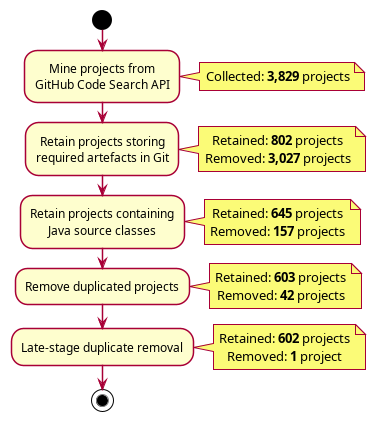
\includegraphics[width=200pt]{figures/data_funnel_diagram.png}
    \caption{Repository selection for the study. A GitHub manifest search on 10 January 2026 returned \num{3829} repositories; source-content filters and duplicate review produced a preliminary corpus of \num{603} repositories and a final corpus of \num{602}. The resulting corpus is the study's identified target population.}
    \label{fig:dataFunnel}
\end{figure}

This mining procedure establishes the population to which the corpus counts refer. The next step defines which files and antipattern occurrences the study measures within that population.

\subsection{Operational scope}\label{sec:antipatternSelection}

We studied static evidence available in Java source code. A relevant file was either generated by jOOQ or contained a reference to jOOQ or a generated class. The first group carried database-design evidence. The second group identified source that directly constructed queries or used generated database objects. This definition excluded Java files with no observable connection to the analysed database-access representation.

A manually maintained path list removed generated files that did not contribute evidence for antipattern detection, including records and plain data objects. It also removed classes generated from database entities outside the application, such as system schemas and tables managed by database extensions. These exclusions kept repository size and annotation effort tied to source that could contain an in-scope occurrence. We analysed source-represented schema and query patterns without building or executing the repositories.

The annotation codebook began with 19 antipatterns from \nobreaktextcite{karwin2023sql}. We excluded concepts that require runtime performance evidence, organisational practice, or framework-level exception behaviour. Index Shotgun provides a concrete boundary. Karwin's recommended process for choosing indexes includes measuring query runtime \nobreakcite[pp. 147--152]{karwin2023sql}, evidence that the Java source alone cannot provide. We therefore excluded that class because static structure did not establish index quality.

We restricted Fear of the Unknown to database-design occurrences and null-unsafe query conditions whose values were visible in the analysed source. For Implicit Columns, the codebook covered jOOQ convenience methods that fetch every column of a table \nobreakcite{jooq2025select}. These calls have the same operational feature as an SQL \texttt{SELECT *}. The projection leaves the required columns unspecified. Online Resource~1 provides the full codebook, exclusions, and decision trees.

Downstream experiments used the seven classes defined in Table~\ref{tab:evaluatedAntipatterns}. This restriction followed the support rule described below and kept the detector evaluation within classes represented across several sampled projects.

\subsection{Sampling, reference annotation, and reliability}\label{sec:referenceAnnotations}

The reference sample came from the preliminary \num{603}-repository corpus. Repository size was the number of relevant files under the definition above. The observed distribution was positively skewed. Most repositories contained few relevant files, whereas a small group contained substantially more. A simple random sample could therefore concentrate annotation effort in the numerous small repositories or select a few large repositories that dominated the reviewed source. We used size strata to retain projects from different parts of this observed distribution.

We formed the strata with two recursive mean splits. The mean relevant-file count across all \num{603} repositories set the first breakpoint. We then calculated the mean among repositories above that breakpoint to set the second. The resulting breakpoints of \num{31} and \num{94} relevant files classified \num{467} repositories as small, \num{100} as medium, and \num{36} as large. These fixed groups describe the preliminary corpus used when the sample was drawn.

We sampled \qty{10}{\percent} from each stratum. With pseudorandom seed \num{123456}, this selected \num{47} small, \num{10} medium, and \num{4} large repositories. The resulting \num{61}-repository sample kept its stratum weights close to those of the preliminary corpus.\label{sec:sampleGeneration}

One annotator with prior jOOQ and SQL-antipattern experience manually reviewed the source code in the \num{61} sampled repositories. The annotator recorded the review in a spreadsheet that was later converted to comma-separated values. Each reference-annotation record identified the antipattern class and repository. It also stored the file path relative to the repository root, the inclusive start and end lines of the occurrence, and a short note about the decision. Class and exact span later provided the comparison unit for repeat annotation and detector evaluation. The file path and repository kept identical line ranges in different files or projects distinct.

The annotator developed a codebook as decision flowcharts while reviewing the sample. Each flowchart translated a class definition into a sequence of source-level decisions. When a previously unseen variant or a non-occurrence edge case exposed a missing rule, the annotator revised the corresponding flowchart and reviewed earlier files that the change could affect. This process applied revised rules throughout the sample.

The completed review produced \num{1562} reference occurrences across the 19 initially included classes. The seven classes retained for detector evaluation account for \num{1436} of those occurrences.

We measured temporal repeatability after a 30-day washout period. Using pseudorandom seed \num{123456}, we sampled \qty{10}{\percent} of files with at least one reference annotation and added an equal number of files without annotations. The latter group tested whether a repeated pass would introduce events in files previously judged negative. The procedure selected \num{128} files, which the same annotator reviewed with the same codebook.

We compared the original and repeated records by antipattern class and exact line span. The two passes contained \num{158} and \num{149} events, respectively, of which \num{142} matched exactly. Treating the original pass as reference gives precision \num{0.953}, recall \num{0.899}, and F1 \num{0.925}. Exact matching requires agreement on the class and both span boundaries, so near-overlapping spans count as disagreements in this check. The exercise measures within-annotator stability; independent annotation and adjudication were unavailable.

\subsection{Project-disjoint partitioning}\label{sec:dataSplit}

We assigned complete repositories to training, validation, and test sets to prevent files from one project appearing in more than one stage. The training set supported iterative prompt development and supplied examples for Few-Shot prompts. The validation set supported comparison and selection of models and prompting strategies after that development. The test set remained held out until the resulting detector configuration was fixed. These roles kept the reported held-out evaluation separate from both prompt construction and configuration selection.

Whole-project assignment was required because files in one repository can share generated schema classes, query idioms, and project-specific support code. Splitting such files among stages would place closely related source in development and evaluation partitions. Assigning all files from a repository together gave \num{21}, \num{20}, and \num{20} projects to training, validation, and test, respectively.

Class and split selection used the complete \num{61}-repository annotation set. Before searching for a split, we retained classes with at least \num{25} occurrences in at least three projects. Twelve of the 19 annotated classes failed this support rule, leaving seven classes for subsequent experiments. The threshold removed classes whose few events or projects could not be distributed meaningfully across three project-disjoint partitions.

We then evaluated all \num{1000000} integer seeds from \num{0} through \num{999999}. Each seed assigned \num{21}, \num{20}, and \num{20} complete projects to the three sets. For each candidate, the objective measured variation in each class's occurrence counts across the splits and summed the squared values over the seven classes. Seed \num{767573} achieved the lowest score, \num{0.52}. This procedure used annotation labels to choose both the retained classes and the split. Table~\ref{tab:trainingTestValidationSplit} reports occurrence and repository support for the resulting partitions.

\begin{table}[tbp]
    \centering
    \small
    \caption{Occurrence and repository support in the project-disjoint split. The partitions contain \num{21} training, \num{20} validation, and \num{20} test repositories. Partition cells give occurrences followed by repositories in parentheses; Total gives occurrences across all partitions. Several classes occur in only one to five projects per partition.}
    \label{tab:trainingTestValidationSplit}
    \begin{tabular}{lrrrr}
        \hline
        \textbf{Class} & \textbf{Total} & \textbf{Training} & \textbf{Validation} & \textbf{Test} \\
        \hline
        Implicit Columns & 795 & 175 (20) & 350 (19) & 270 (20) \\
        ID Required & 259 & 55 (18) & 99 (15) & 105 (16) \\
        Keyless Entry & 122 & 30 (7) & 56 (1) & 36 (3) \\
        Fear of the Unknown & 95 & 23 (6) & 36 (8) & 36 (5) \\
        31 Flavors & 71 & 17 (6) & 15 (4) & 39 (1) \\
        Poor Man's Search Engine & 55 & 19 (5) & 15 (4) & 21 (3) \\
        Rounding Errors & 39 & 13 (4) & 10 (1) & 16 (2) \\
        \hline
    \end{tabular}
\end{table}

The data-dependent support rule and seed search balanced occurrence counts. Whole-project assignment prevented direct file-level overlap. Several classes still had only one to five projects per partition.

\subsection{Detector configuration and execution}\label{sec:experimentsQuantitative}

We limited each detector invocation to one request and one response. This scope allowed the same execution structure to cover four prompting strategies without adding multi-turn state. We developed universal prompts against the training partition and compared revisions with its reference annotations across the evaluated models. We performed no model-specific tuning.

Zero-Shot and Few-Shot followed established prompting designs \nobreakcite{DBLP:journals/csur/LiuYFJHN23,DBLP:conf/nips/BrownMRSKDNSSAA20}. Chain-of-Thought and Tree-of-Thought-inspired prompts elicited explicit intermediate analysis \nobreakcite{DBLP:conf/nips/KojimaGRMI22,DBLP:conf/nips/Wei0SBIXCLZ22,tree-of-thought-prompting,DBLP:conf/nips/YaoYZS00N23}. Each configuration used two prompts. One prompt examined non-generated source for query antipatterns, and the other examined jOOQ-generated source for database-design antipatterns. The request for generated source also received the closest generated key-definition class. Its primary, unique, and foreign-key definitions supplied the schema context needed to judge whether a Keyless Entry candidate had a suitable referenced key.

Before submission, we removed leading and trailing whitespace from every source line to reduce input size. We then prefixed each line with its original line number so the response could refer to spans in the unmodified file. Each response used structured fields for class, span, code fragment, and explanation. These transformations gave every configuration the same source and output representation.

Prompt development began with broad class instructions that left more of each decision to the model. During comparison with the training reference annotations, we found cases where the returned interpretation differed from the study's codebook. We therefore made each operational definition explicit and added relevant method calls, coding patterns, and exclusions where the class name alone did not determine the intended rule. The resulting instructions stated the intended decision boundary in the same terms as the annotation codebook.

Localisation rules became more specific through the same process. For ID Required, 31 Flavors, Poor Man's Search Engine, and Implicit Columns, the prompt stated which lines of a larger expression belonged to the returned occurrence. These instructions separated the class decision from the span decision, both of which affect occurrence-level agreement. Few-Shot prompts drew examples from the training partition when it contained the required variant. We created synthetic examples for variants and edge cases absent from that partition. Online Resource~1 provides the preserved prompt templates and localisation rules.\label{sec:prompts}

The model set varied in size, reasoning mode, and weight availability. Each model offered stable weights or a point-in-time snapshot and accepted structured outputs conforming to the requested JSON Schema. We applied the same prompts to open- and closed-weight models and to configurations with reasoning enabled or disabled.

The selected set comprised OpenAI GPT-5.2 \nobreakcite{gpt52}, Z.ai GLM-5 \nobreakcite{DBLP:journals/corr/abs-2602-15763}, Anthropic Claude Opus 4.5 \nobreakcite{opus45Card}, and OpenAI gpt-oss-120B \nobreakcite{DBLP:journals/corr/abs-2508-10925}.

We compared these four models and four prompting configurations on the \num{20}-repository validation set, originally reported as containing \num{823} relevant files. Surviving notebook copies process \num{1159} files, and the exact outputs underlying the originally reported comparison are unavailable. Validation requests used the OpenAI Python SDK \nobreakcite{openAiPython2026GitHub} through OpenRouter \nobreakcite{openRouter2026homepage}. GPT-5.2 used xhigh reasoning, which did not support temperature adjustment. Archived requests nevertheless submitted temperature \num{0.0} to the gateway, whose handling of that field was not recorded. GLM-5 used temperature \num{0.0}, and its reasoning effort was not configurable. Claude Opus 4.5 used temperature \num{0.0} with reasoning disabled. We retained the default temperature of \num{1.0} for gpt-oss-120B with high reasoning because near-zero temperatures caused repeated-token loops. We ran each model-prompt pair once and selected the final configuration by observed agreement, cost, and runtime.\label{sec:models}

OpenAI Codex with GPT-5.4 \nobreakcite{gpt54} assisted implementation of the detector under human-defined requirements, review, and acceptance. The final detector recursively selected relevant Java files, attached key-definition context where available, submitted a structured request for each file, retried failures, and retained each returned class-labelled span. We executed one primary run on the \num{20} held-out projects, targeting \num{502} relevant files. The run cost \usd{14.34}, took \num{386} seconds, and returned \num{536} predictions. The corpus execution was recorded as using the same model, settings, and Zero-Shot prompt family. It produced the flags used for RQ2 and the exploratory source-fragment analysis.

Dashboard records date the archived Zero-Shot, Few-Shot, and Chain-of-Thought runs to 6 and 7 March 2026 and the Tree-of-Thought-inspired runs to 27 March. The held-out and corpus executions are dated 4 and 15 April 2026, respectively. Validation notebooks retried empty or failed responses. GLM-5 requests fixed Friendli as the backend and disabled provider fallbacks. Comparable routing records for the other models are unavailable. The held-out command allowed up to \num{1000} retries per file, with no additional attempts in the dashboard total. The corpus command allowed two retries per file. The \href{https://github.com/kristoisberg/thesis-paper/blob/4a3b4d55073adbb38325ca43872852d2a75649c9/analysis/README.md\#original-model-executions}{replication README} preserves the detailed execution records and their provenance limits.

\subsection{Localisation evaluation and error analysis}

The primary evaluation compares the \num{536} held-out predictions with \num{523} original reference spans. A candidate match must share repository, file, and class. For predicted span $S_p$ and reference span $S_r$, we compute line-level intersection over union (IoU):
\begin{equation}
    \operatorname{IoU}(S_p,S_r)=\frac{|S_p\cap S_r|}{|S_p\cup S_r|}.
\end{equation}
At the primary threshold of \num{0.50}, maximum-cardinality bipartite matching assigns each prediction and reference to at most one pair. Candidate lists are ordered by descending IoU, predicted span, and source order for deterministic tie handling. Matched pairs are true positives, unmatched predictions are false positives, and unmatched references are false negatives.

We calculate precision, recall, and F1 from these event counts for each class. Micro averages pool events across classes, macro averages weight classes equally, and reference-support-weighted averages use each class's reference count. True negatives are undefined for occurrence localisation, so these counts are event matches rather than confusion matrices.

Two robustness procedures test the primary result. First, we repeat the one-to-one matching at IoU thresholds \num{0.25}, \num{0.75}, and \num{1.00}. Second, a project-cluster bootstrap resamples all \num{20} test projects with replacement for \num{10000} iterations using seed \num{123456}. Each draw retains every reference and prediction from a sampled project. The percentile ranges measure how the held-out agreement metrics vary with project composition within the selected split.

We manually reviewed unmatched references and predictions to classify recurring semantic and localisation errors. This detector-informed review produced a revised set of \num{563} reference events. It could miss occurrences absent from both the detector output and original annotations. Because detector disagreements guided the revision, we retain the original annotations as the primary reference and report revised-reference results as an optimistic sensitivity analysis.

\subsection{Corpus measures and exploratory source-fragment coding}\label{sec:corpusMeasures}

The corpus execution covered all \num{602} repositories, including the \num{61} sampled repositories, and produced \num{15931} positive flags. We reconstructed its source frame from the analysis snapshot using the released detector's recursive \path{**/*.java} discovery and file filters, then removed duplicate paths. The resulting frame contains \num{17988} distinct repository-relative relevant file paths: \num{17314} under a \texttt{src} path component, \num{360} under \path{target/generated-sources}, and \num{314} in other source locations. The earlier \num{17450}-file count used a narrower \path{src/**/*.java} scan that emitted \num{136} duplicate paths and omitted \num{674} detector-selected files. We use the reconstructed file-occurrence frame for all file-normalised results.

We assign each selected file one source role. Files containing the detector's generated-table indicators form the \emph{generated schema} role, which contains \num{7226} files. The other \num{10762} selected files form the \emph{application/query source} role. Generated-schema files are eligible for database-design classes, and application/query files are eligible for query classes. Fear of the Unknown spans both representations, so we analyse its two roles separately.

For repository $r$ and class-role pair $c$, let $Y_{rc}$ be the number of flags, $F_{rc}$ the number of eligible files, and $A_{rc}$ the number of eligible files with at least one flag. Flagged-file breadth is $100A_{rc}/F_{rc}$, within-file repetition is $Y_{rc}/A_{rc}$, and flag density is $100Y_{rc}/F_{rc}$. The pooled density divides flags summed across repositories by eligible files summed across repositories. The repository-equal density is the mean of repository densities among repositories with eligible files. Eligible repositories without flags contribute zero; repositories without eligible files have undefined rates and are omitted. We also report an all-class broad density over all relevant files.

To separate repository size from density, we retain all \num{602} repository records and apply the existing total-relevant-file strata: small repositories contain at most \num{31} files, medium repositories contain \numrange{32}{94}, and large repositories contain more than \num{94}. For each class-role frame and for the broad result, we select the ceiling of \qty{10}{\percent} of flagged repositories by flag count, with repository name breaking cutoff ties. We compare that group's shares of flags and eligible files with its density relative to the remaining repositories and report bounds over every possible cutoff-tie selection.

Finally, we test sensitivity to repeated content. A relevant file occurrence belongs to an exact-duplicate group when its SHA-256 appears more than once. Exact-content events are unique by content hash, class, source role, and inclusive line span. We weight each unique content and event once across its physical copies when calculating repository concentration. This procedure covers byte-identical files; modified clones remain outside the sensitivity analysis.

The execution was recorded as using the selected model, settings, and Zero-Shot prompt family. The corpus analysis describes detector output; prevalence and API-specific risk estimates would require an independent audit, class-specific error estimates, and class-specific API-opportunity denominators.

For Implicit Columns and Poor Man's Search Engine, we assigned one exploratory source-fragment category to each detector flag. A fixed, precedence-ordered list of string and regular-expression patterns was applied to the code fragment returned by the detector, with the first matching pattern determining the category. We report leading patterns individually, pool the remaining recurring matches as other categorised patterns, and combine sparse or unmatched fragments in one group. Online Resource~1 provides the ordered patterns.

\section{Results}\label{sec:results}

\subsection{Detector configuration selection}\label{sec:detectorSelectionResults}

Based on the validation comparison in Table~\ref{tab:configurationSelection}, we selected Claude Opus 4.5 \nobreakcite{opus45Card}, with reasoning disabled, temperature \num{0.0}, and the Zero-Shot prompts \nobreakcite{DBLP:journals/csur/LiuYFJHN23}. The comparison also included GPT-5.2, GLM-5, and gpt-oss-120B \nobreakcite{gpt52,DBLP:journals/corr/abs-2602-15763,DBLP:journals/corr/abs-2508-10925}, with Few-Shot, Chain-of-Thought, and Tree-of-Thought-inspired prompts following established designs \nobreakcite{DBLP:conf/nips/BrownMRSKDNSSAA20,DBLP:conf/nips/KojimaGRMI22,DBLP:conf/nips/Wei0SBIXCLZ22,tree-of-thought-prompting,DBLP:conf/nips/YaoYZS00N23}. Three models reported the same displayed reference-support-weighted F1-score of \num{0.88} with Zero-Shot prompts. Claude Opus 4.5 completed the comparison in \num{367} seconds, the shortest runtime among the Zero-Shot configurations. The reasoning-oriented prompts reached \num{0.90} F1 with higher costs and runtimes. We therefore selected the simpler configuration for the held-out and corpus runs.

\begin{table}[tbp]
    \centering
    \scriptsize
    \caption{Validation results used to select the detector configuration. Precision, recall, and F1 are reference-support-weighted occurrence-agreement metrics over \num{20} validation repositories. Costs are reported by OpenRouter in US dollars, and runtime is in seconds. The first four rows compare models with Zero-Shot prompts; the final three compare alternative prompts with Claude Opus 4.5.}
    \label{tab:configurationSelection}
    \begin{tabular}{llrrrrr}
        \hline
        \textbf{Model} & \textbf{Prompt} & \textbf{P} & \textbf{R} & \textbf{F1} & \textbf{Cost (USD)} & \textbf{Time (s)} \\
        \hline
        GPT-5.2 & Zero-Shot & 0.85 & 0.92 & 0.88 & 26.16 & 2423 \\
        GLM-5 & Zero-Shot & 0.88 & 0.89 & 0.88 & 11.76 & 5774 \\
        Claude Opus 4.5 & Zero-Shot & 0.88 & 0.89 & 0.88 & 31.39 & 367 \\
        gpt-oss-120B & Zero-Shot & 0.83 & 0.87 & 0.83 & 1.49 & 2808 \\
        Claude Opus 4.5 & Few-Shot & 0.88 & 0.89 & 0.88 & 45.00 & 352 \\
        Claude Opus 4.5 & Chain-of-Thought & 0.92 & 0.90 & 0.90 & 40.86 & 956 \\
        Claude Opus 4.5 & Tree-of-Thought & 0.92 & 0.90 & 0.90 & 81.43 & 4701 \\
        \hline
    \end{tabular}
\end{table}

\subsection{RQ1: What occurrence-level agreement does the selected detector achieve on held-out jOOQ projects?}\label{sec:rq1Agreement}

In one run, the selected detector returned \num{536} predictions from \num{502} relevant files in the \num{20}-repository test partition. The original reference contained \num{523} spans. At the prespecified intersection-over-union threshold of \num{0.50}, the one-to-one matching procedure yielded \num{460} true positives, \num{76} false positives, and \num{63} false negatives. The corresponding micro precision, recall, and F1-score were \num{0.858}, \num{0.880}, and \num{0.869}.

Table~\ref{tab:toolDetections} shows that the aggregate result masks substantial class differences. F1-scores ranged from \num{0.481} for Fear of the Unknown to \num{0.974} for 31 Flavors. Implicit Columns, 31 Flavors, and Rounding Errors each exceeded \num{0.89}, whereas Keyless Entry, Fear of the Unknown, and Poor Man's Search Engine remained below \num{0.70}. The macro precision, recall, and F1-score were \num{0.797}, \num{0.813}, and \num{0.793}; the reference-support-weighted values were \num{0.885}, \num{0.880}, and \num{0.877}. These aggregates reinforce the need to interpret each corpus flag class in light of its own held-out agreement.

\begin{table}[H]
    \centering
    \small
    \caption{Occurrence-level agreement with the original reference spans at intersection over union \num{0.50}. True positives (TP), false positives (FP), and false negatives (FN) are one-to-one event-matching counts; true negatives are undefined for this localisation task. The final row pools all classes.}
    \label{tab:toolDetections}
    \begin{tabular}{lrrrrrr}
        \hline
        \textbf{Antipattern} & \textbf{TP} & \textbf{FP} & \textbf{FN} & \textbf{Precision} & \textbf{Recall} & \textbf{F1} \\
        \hline
        Implicit Columns & 253 & 4 & 17 & 0.984 & 0.937 & 0.960 \\
        ID Required & 89 & 13 & 16 & 0.873 & 0.848 & 0.860 \\
        Keyless Entry & 35 & 30 & 1 & 0.538 & 0.972 & 0.693 \\
        Fear of the Unknown & 19 & 24 & 17 & 0.442 & 0.528 & 0.481 \\
        31 Flavors & 38 & 1 & 1 & 0.974 & 0.974 & 0.974 \\
        Poor Man's Search Engine & 13 & 4 & 8 & 0.765 & 0.619 & 0.684 \\
        Rounding Errors & 13 & 0 & 3 & 1.000 & 0.813 & 0.897 \\
        \textbf{Micro total} & \textbf{460} & \textbf{76} & \textbf{63} & \textbf{0.858} & \textbf{0.880} & \textbf{0.869} \\
        \hline
    \end{tabular}
\end{table}

\subsubsection{Class-specific errors}\label{sec:detectionErrors}

The disagreements in Table~\ref{tab:detectionErrors} cluster around local query semantics, inferred relationships, missing-value conventions, and occurrence grouping. Inspection also exposed omissions and span errors in the original reference annotations. Because detector disagreements guided this review, the primary result retains the original reference.

\begin{table}[tbp]
    \centering
    \small
    \caption{Dominant disagreement mechanisms observed during qualitative review of the held-out run. Counts refer to false positives or false negatives against the original reference spans.}
    \label{tab:detectionErrors}
    \begin{tabular}{p{2.9cm}p{7.8cm}}
        \hline
        \textbf{Antipattern} & \textbf{Observed disagreement mechanisms} \\
        \hline
        Implicit Columns & Fourteen of \num{17} false negatives used \texttt{returning()} or \texttt{returningResult()}. Other disagreements involved span boundaries and reference errors. \\
        ID Required & Six false negatives involved primary-key columns named \texttt{id}. One false positive proposed an unsuitable natural key; other disagreements exposed reference errors. \\
        Keyless Entry & Fifteen of \num{30} false positives involved audit-log tables, which the prompt did not exempt. One involved an ambiguous column name, and the remainder included missing or disputed reference annotations. \\
        Fear of the Unknown & All \num{17} false negatives involved defaults or sentinel values. Of \num{24} false positives, \num{23} exposed omissions in the original reference and one suggested a refactoring rather than an occurrence. \\
        31 Flavors & One false negative involved a numeric \texttt{CHECK} range encoding categories. The single false positive inferred a fixed value set from a \texttt{status} column without supporting schema evidence. \\
        Poor Man's Search Engine & Seven false negatives and two false positives resulted from grouping consecutive occurrences into one span. Two false positives used \texttt{LIKE} without wildcards, and one false negative placed \texttt{containsIgnoreCase} in an intermediate collection. \\
        Rounding Errors & All three false negatives involved \texttt{DOUBLE} coefficients later used to calculate monetary winnings. \\
        \hline
    \end{tabular}
\end{table}

Four mechanisms dominated: all-column \texttt{returning()} calls, keyless audit logs, sentinel defaults, and grouped search expressions. The remaining disagreements mainly involved line boundaries, sparse schema evidence, or class-specific semantics already summarised in the table.

The detector-informed revision contained \num{563} reference spans and changed the pooled totals to \num{512} true positives, \num{24} false positives, and \num{51} false negatives. These totals yield micro precision \num{0.955}, recall \num{0.909}, and F1-score \num{0.932}. We treat this result as an optimistic sensitivity analysis.

Micro F1 varied by \num{0.010} across the tested span boundaries. Table~\ref{tab:iouSensitivity} reports the complete threshold grid.

\begin{table}[tbp]
    \centering
    \small
    \caption{Sensitivity of pooled occurrence-level agreement to the line-span intersection-over-union (IoU) threshold. True positives (TP), false positives (FP), and false negatives (FN) follow the same one-to-one matching rule for all \num{536} predictions and \num{523} original reference spans. Micro F1 ranges from \num{0.863} to \num{0.873}.}
    \label{tab:iouSensitivity}
    \begin{tabular}{rrrrrrr}
        \hline
        \textbf{IoU} & \textbf{TP} & \textbf{FP} & \textbf{FN} & \textbf{Precision} & \textbf{Recall} & \textbf{F1} \\
        \hline
        0.25 & 462 & 74 & 61 & 0.862 & 0.883 & 0.873 \\
        0.50 & 460 & 76 & 63 & 0.858 & 0.880 & 0.869 \\
        0.75 & 457 & 79 & 66 & 0.853 & 0.874 & 0.863 \\
        1.00 & 457 & 79 & 66 & 0.853 & 0.874 & 0.863 \\
        \hline
    \end{tabular}
\end{table}

Only Implicit Columns and Poor Man's Search Engine changed across these thresholds. The pooled score remained within the \num{0.863}--\num{0.873} range.

A \num{10000}-replicate project-cluster bootstrap placed micro precision between \num{0.798} and \num{0.931}, micro recall between \num{0.820} and \num{0.913}, and micro F1 between \num{0.820} and \num{0.912}. These percentile ranges describe sensitivity to the composition of the selected test projects.

\subsection{RQ2: How are the selected detector's flags distributed across the seven SQL antipatterns, eligible files, and repositories in the 602-repository corpus, including recurring source-fragment patterns for two query classes?}\label{sec:rq2CorpusFlags}

The corpus source frame contains \num{17988} relevant file occurrences in \num{602} repositories, and the detector produced \num{15931} positive flags. At least one retained class was flagged in \num{7653} files, or \qty{42.5}{\percent}, and \num{601} repositories, or \qty{99.8}{\percent}.

\begin{table}[H]
    \centering
    \scriptsize
    \setlength{\tabcolsep}{2pt}
    \caption{Selected-detector output in the identified \num{602}-repository corpus. G denotes the \num{7226} generated-schema files and A the \num{10762} application/query files; All contains \num{17988} relevant file occurrences. Repository coverage and file breadth give counts followed by percentages in parentheses. The two Fear of the Unknown repository counts overlap in two repositories. Repetition is flags per flagged file. Pooled and repository-equal densities are flags per 100 eligible files; the latter gives each eligible repository equal weight and includes zero-flag repositories.}
    \label{tab:corpusFlags}
    \begin{tabular}{lrrrrr}
        \hline
        \makecell[l]{\textbf{Antipattern}\\\textbf{and role}} & \textbf{Flags} & \makecell{\textbf{Repository}\\\textbf{coverage}} & \makecell{\textbf{File}\\\textbf{breadth}} & \makecell{\textbf{Repeti-}\\\textbf{tion}} & \makecell{\textbf{Density}\\\textbf{pooled / repo.}} \\
        \hline
        Implicit Columns (A) & 7289 & 535 (88.9) & 2607 (24.2) & 2.80 & 67.73 / 92.63 \\
        ID Required (G) & 3597 & 523 (86.9) & 3591 (49.7) & 1.00 & 49.78 / 59.90 \\
        Keyless Entry (G) & 2153 & 200 (33.2) & 1269 (17.6) & 1.70 & 29.80 / 17.76 \\
        Fear of the Unknown (G) & 1240 & 197 (32.7) & 675 (9.3) & 1.84 & 17.16 / 20.59 \\
        Fear of the Unknown (A) & 16 & 10 (1.7) & 11 (0.1) & 1.45 & 0.15 / 0.17 \\
        31 Flavors (G) & 390 & 87 (14.5) & 292 (4.0) & 1.34 & 5.40 / 4.70 \\
        \makecell[l]{Poor Man's Search Engine (A)} & 583 & 114 (18.9) & 319 (3.0) & 1.83 & 5.42 / 4.27 \\
        Rounding Errors (G) & 663 & 86 (14.3) & 343 (4.7) & 1.93 & 9.18 / 7.63 \\
        \textbf{Any retained class (All)} & \textbf{15931} & \textbf{601 (99.8)} & \textbf{7653 (42.5)} & \textbf{2.08} & \textbf{88.56 / 93.63} \\
        \hline
    \end{tabular}
\end{table}

Table~\ref{tab:corpusFlags} separates class totals, repository coverage, flagged-file breadth, within-file repetition, and density in the corresponding source-role frame. The two most frequent classes have different output structures. ID Required flags cover \num{3591} of \num{7226} generated-schema files, or \qty{49.7}{\percent}, and average \num{1.00} per flagged file. Implicit Columns flags cover \num{2607} of \num{10762} application/query files, or \qty{24.2}{\percent}, and average \num{2.80} flags per flagged file. The first class is therefore broader across its eligible file frame, whereas the second repeats more within flagged files. Implicit Columns and ID Required together account for \num{10886} flags, or \qty{68.3}{\percent} of the output.

Across all repositories, pooled density is \num{88.56} flags per 100 relevant files. The repository-equal mean is \num{93.63}, and the median is \num{83.46}, with an interquartile interval of \numrange{51.28}{120.00}. Raw flag count correlates with relevant-file count at Spearman $\rho=\num{0.778}$. Large repositories contain \qty{43.8}{\percent} of relevant files and \qty{39.8}{\percent} of flags. Their broad density is \num{80.50}, below the small- and medium-repository densities of \num{93.19} and \num{96.65}.

Repository size therefore explains part of the raw concentration. The 61 highest-count repositories contain \qty{59.1}{\percent} of all flags and \qtyrange{48.1}{49.6}{\percent} of relevant files across the three-way cutoff tie. Their density is \numrange{1.47}{1.56} times that of the remaining repositories. High-count repositories combine greater file volume with higher density, while the large stratum as a whole has the lowest pooled density.

Exact-content sensitivity preserves both headline results. Of the \num{17988} file occurrences, \num{1109}, or \qty{6.17}{\percent}, belong to \num{488} exact-duplicate groups and contain \num{1080}, or \qty{6.78}{\percent}, of the raw flags. The groups contain \num{621} copies beyond their first occurrences. Taking the union of class-and-span events across byte-identical copies yields \num{15355} exact-content events over \num{17367} unique contents. Eight groups have inconsistent event sets, but selecting one physical representative from each group yields \numrange{15340}{15349} events without changing the interpretation. ID Required remains broader with almost no repetition, and Implicit Columns remains narrower and repetitive. The highest-count decile contains \qty{59.4}{\percent} of exact-content events, \qtyrange{50.1}{50.3}{\percent} of eligible unique-content weight, and \numrange{1.44}{1.46} times the remaining density. Byte-identical copies therefore do not explain the conclusions.

\subsubsection{Exploratory source-fragment strata}\label{sec:fragmentStrata}

Table~\ref{tab:apiManifestations} groups recurring source-fragment patterns among Implicit Columns and Poor Man's Search Engine flags. The two leading Implicit Columns patterns both selected all fields from a table. Together, they contained \num{5227} of \num{7289} flags, or \qty{71.7}{\percent}. Explicit field-array and asterisk patterns contributed a further \num{945} flags, or \qty{13.0}{\percent}. Named recurring categories accounted for \qty{94.1}{\percent} of the class flags.

For Poor Man's Search Engine, fragments matching \texttt{like(} contained \num{273} of \num{583} flags, or \qty{46.8}{\percent}. The next three patterns matched case-insensitive or contains-style method names. These four categories contained \num{517} flags, or \qty{88.7}{\percent}. Named recurring categories accounted for \qty{93.7}{\percent}.

\begin{table}[H]
    \centering
    \small
    \caption{Exploratory source-fragment categories among detector flags for two query antipatterns. Categories use precedence-ordered string or regular-expression matches over detector-returned code fragments. Shares use each class's total flag count as denominator.}
    \label{tab:apiManifestations}
    \begin{tabular}{p{2.2cm}p{5.3cm}rr}
        \hline
        \textbf{Flag class} & \textbf{Source-fragment category} & \textbf{Flags} & \textbf{Share (\%)} \\
        \hline
        \makecell[l]{Implicit\\Columns} & \texttt{selectFrom} fragment & 3417 & 46.9 \\
        & \texttt{select()} fragment & 1810 & 24.8 \\
        & \texttt{fields()} fragment & 665 & 9.1 \\
        & \texttt{asterisk()} fragment & 280 & 3.8 \\
        & Other categorised patterns & 688 & 9.4 \\
        & Sparse matched or uncategorised & 429 & 5.9 \\
        \hline
        \makecell[l]{Poor Man's\\Search Engine} & \texttt{like(} fragment & 273 & 46.8 \\
        & \texttt{containsIgnoreCase(} fragment & 96 & 16.5 \\
        & \texttt{likeIgnoreCase(} fragment & 87 & 14.9 \\
        & \texttt{contains(} fragment & 61 & 10.5 \\
        & Other categorised patterns & 29 & 5.0 \\
        & Sparse matched or uncategorised & 37 & 6.3 \\
        \hline
    \end{tabular}
\end{table}

\section{Discussion}\label{sec:discussion}

The findings suggest that interpreting detector output requires both class-specific validation and an account of where flags occur. Agreement identifies the kinds of decisions that require closer inspection. File breadth, within-file repetition, and repository density describe the scope of that inspection. Together, these results inform how the detector could support code review and how its corpus output should be independently audited.

\subsection{Interpreting flags by antipattern class}

The pooled agreement score provides an incomplete basis for deciding how to use a finding. Implicit Columns and ID Required contribute \qty{68.3}{\percent} of corpus flags, but their held-out disagreement mechanisms differ from those of other classes. Table~\ref{tab:toolDetections} reports precision \num{0.984} for Implicit Columns and \num{0.538} for Keyless Entry against the original reference. These observations motivate different review questions for the two classes. For Implicit Columns, the reviewer can inspect the selected projection and its consumers. For Keyless Entry, the reviewer must establish whether a column represents a relationship that should be enforced by a foreign key.

The Keyless Entry disagreements illustrate how an operational definition can leave a contextual decision unresolved. Half of its apparent false positives involved audit-log tables that the prompt did not exempt. Deciding whether such a table should retain a foreign-key constraint requires understanding its intended behaviour. A matching column name and a suitable referenced key provide evidence for a possible relationship, but the reviewer still needs to assess the application's requirements. This makes the class a candidate for explicit review of exceptions before accepting a proposed schema change.

Fear of the Unknown shows why disagreement also requires scrutiny of the reference. Of its \num{24} apparent false positives, \num{23} exposed omissions in the original annotations. Its low F1 therefore combines missed reference occurrences with incomplete annotation coverage. All \num{17} false negatives involved defaults or sentinel values. These findings identify two needs for further validation: independent annotation of missing-value conventions and targeted inspection of the source forms the detector missed. The detector-informed revision helps locate these issues, but independent review is needed to establish how often each occurs beyond the test set.

The search-class disagreements raise a separate question about the unit of a finding. Grouping consecutive search expressions into one predicted span produced most of the false negatives for Poor Man's Search Engine. A reviewer may see the relevant code in that span, yet the occurrence counts differ from a reference that marks each expression separately. The modest sensitivity to overlap thresholds in Table~\ref{tab:iouSensitivity} suggests that changing the matching boundary alone would leave much of this problem unresolved. A review interface could retain the enclosing query as context while presenting each search expression as a separate finding.

Class-specific validation thus supplies questions for reviewing corpus output. Projection semantics, intended relationships, missing-value conventions, and occurrence grouping each call for different evidence. The held-out results identify these priorities; measuring their frequency in the wider corpus requires an independent sample of that corpus.

\subsection{Implications for reviewing repositories}

File breadth and within-file repetition imply different scopes for inspection. ID Required flags cover almost half of the generated-schema files and average about one flag per flagged file. Implicit Columns flags cover about one quarter of application/query files and average nearly three flags per flagged file. The first pattern suggests review across many schema definitions. The second suggests reviewing several query expressions together within a smaller share of application files. A queue ordered only by total class count would hide this distinction.

For ID Required, the relevant review context is the underlying table definition and its candidate keys. Under the operational definition in Table~\ref{tab:evaluatedAntipatterns}, a primary key named \texttt{id} is sufficient for a flag. The reported breadth therefore depends partly on that definition's treatment of a naming choice. The reviewer must still determine whether the key design is appropriate and whether a proposed natural or compound key meets the application's requirements. The observed file coverage describes how widely the detector applies this rule; the study does not measure the consequences of the flagged designs.

For Implicit Columns, repeated findings within one file make the use of fetched records a useful review context. A reviewer could inspect whether the affected expressions need every selected field, how their results are consumed, and which explicit projections would preserve behaviour. Reviewing the expressions together may reveal a shared query-construction convention. That possibility would need to be checked in the source before treating multiple flags as one refactoring task. The repetition measure identifies where such an inspection could be useful without establishing that the flagged expressions have a common cause.

Repository counts likewise support several distinct inspection goals. High raw counts identify repositories contributing many findings to the corpus. File-normalised density identifies repositories producing more flags relative to their relevant-file volume. The highest-count group combines about half of the relevant files with approximately one and a half times the density of the remaining repositories. However, the large-repository stratum as a whole has lower pooled density than the smaller strata. Selecting repositories by raw count and selecting them by density therefore address different inspection goals.

These measures can guide the allocation of review effort, but an assessment of remediation priority would also require the validity and consequences of individual findings. Pooling classes gives each flag equal weight even though their definitions and review requirements differ. Class-specific breadth and density provide a more informative starting point for inspection. Exact-content sensitivity preserves the main breadth, repetition, and concentration patterns, supporting their use in planning an audit that also checks modified clones and related code.

\subsection{Priorities for independent corpus validation}

The source-fragment categories provide a concrete starting point for an independent audit. In Table~\ref{tab:apiManifestations}, \texttt{selectFrom} and \texttt{select()} fragments together contain \qty{71.7}{\percent} of Implicit Columns flags, and \texttt{like(} fragments contain \qty{46.8}{\percent} of Poor Man's Search Engine flags. Sampling these categories would cover a substantial share of the returned output. An audit should also include the remaining categories and source forms absent from the flagged fragments, so that its conclusions extend beyond the most visible detector findings.

For Implicit Columns, the held-out errors identify an additional sampling priority. Fourteen of the \num{17} missed occurrences used an all-column returning clause, expressed through \texttt{returning()} or \texttt{returningResult()}. These calls should be examined alongside the common flagged projection forms. An independent source inventory could identify eligible expressions, resolve their call targets, and record whether the detector flagged each one. Review of flagged expressions would assess agreement with the class definition; review of unflagged expressions would reveal missed occurrences. Both are needed to estimate corpus precision and recall.

For Poor Man's Search Engine, the audit must distinguish confirmed full-text matching, excluded prefix searches, expressions without wildcards, and cases whose arguments leave the wildcard behaviour unresolved. The operational definition includes the last category conservatively. An audit should record those cases separately so that uncertainty about a search expression remains visible in the findings. Consecutive conditions should also be annotated individually, with their enclosing query retained as context. This would separate decisions about search semantics from disagreements about occurrence grouping.

The sampling frame must come from the source corpus. The current fragment categories use precedence-ordered matches over detector-returned text, so their shares describe the composition of flags. An independent inventory of eligible API uses would provide the denominator needed to compare how often different source forms are flagged or missed. Sampling should span repositories and include unflagged uses, with independent annotations and adjudication of disputed cases. Such an audit would test whether the class-specific agreement observed in the held-out projects carries over to the corpus and whether the dominant fragment categories remain dominant among independently confirmed occurrences.

The same independently annotated material could support a deterministic baseline for the jOOQ task. Rules over resolved calls or an abstract syntax tree could target explicitly represented conditions, following established rule-based detection approaches \nobreakcite{DBLP:journals/tse/MohaGDM10}. Candidate rules include all-column projections and the primary-key naming condition used for ID Required. Contextual decisions about suitable keys, audit-log relationships, or semantically meaningful sentinels would require additional evidence. Evaluating these rules on the same files, operational definitions, and occurrence-matching procedure would establish their coverage and compare agreement, cost, and runtime with the LLM detector. The resulting error analysis could then identify which decisions benefit from model-based interpretation and which can be handled by explicit rules.

\section{Threats to Validity}\label{sec:limitations}

\subsection{Construct validity}

The seven antipattern classes follow study-specific operational definitions derived from Karwin's catalogue \nobreakcite{karwin2023sql}. Different boundaries for sentinel values, implicit projections, search patterns, or inferred keys would change the counts. Agreement with the single-annotator reference therefore measures conformance to these definitions and one annotator's application of them, without independent consensus on annotation correctness.

The primary matching rule treats class-labelled line spans as events and requires one-to-one overlap at intersection over union \num{0.50}. It captures class, occurrence count, and approximate localisation, but may count grouping differences as errors even when the detector identifies the same problematic code. True negatives are undefined, and the threshold analysis tests robustness only to the chosen span boundary.

The corpus measures use role-eligible files as denominators rather than class-specific opportunities for an antipattern. For example, an application/query file may contain no eligible projection or search predicate. They also retain detector errors observed in the held-out evaluation. The exploratory categories classify returned fragments without resolving call targets. Accordingly, the corpus results characterise detector-output density, breadth, repetition, and fragment composition. Estimating antipattern prevalence or API risk would require an independent audit with API-opportunity denominators.

The exact-content sensitivity identifies byte-identical files by SHA-256. Modified clones can still receive repeated weight, and repositories may share related code whose bytes differ. The unchanged exact-content results bound the effect of exact copies alone.

\subsection{Internal validity}

The primary evaluation retains the original annotations, whereas the sensitivity analysis revised records after inspecting detector disagreements. This process favours errors visible to the detector and can miss shared omissions. The revised-reference result is therefore optimistic.

Class retention and project partitioning were data-dependent. The support rule used the complete \num{61}-repository annotation set, and the split was selected from \num{1000000} seeds using per-class occurrence balance. Project-disjoint assignment prevents file overlap, but the retained classes and split composition remain adapted to the observed sample.

The preliminary sampling frame contained one duplicate repository and an incomplete path list for excluding irrelevant generated files. These conditions remain part of the sample and partitions. Later analysis stages corrected the file counts and retained all \num{15931} detector flags. An overbroad \path{mysql/tables} exclusion skips an annotated application table in the test partition. Model and prompt selection also used one validation partition and one observed run per configuration, making the choice sensitive to that partition and execution.

\subsection{External validity}

The target population comes from a dated GitHub search and its filters. The frame may exclude software outside GitHub, projects without the required build declarations or retained generated jOOQ classes, and repositories omitted when a query exceeded the API's \num{1000}-result cap. The \num{602}-repository results therefore apply to this identified population.

All analysed repositories are open source, and proprietary systems may differ in schema scale, coding conventions, review practice, and domain. The detector covers seven of the original 19 codebook classes in Java jOOQ code. Excluded classes, other query builders, and runtime-only manifestations may behave differently.

The corpus includes all \num{61} sampled repositories and is therefore not an independent transfer population. Repositories outside the sample lack reference annotations, and the corpus has no independent audit. Held-out agreement may change on source forms absent from the reference sample.

\subsection{Conclusion validity}

The held-out reference is imbalanced across classes and projects. As Table~\ref{tab:trainingTestValidationSplit} shows, Implicit Columns contributes \num{270} of the \num{523} reference occurrences, and several classes have support in only one to five test repositories. The micro aggregate is dominated by Implicit Columns. Sparse class estimates are sensitive to individual projects.

The project-cluster bootstrap preserves within-project dependence, but its percentile range is conditional on the label-informed \num{20}-project partition. It is neither a population confidence interval nor an estimate of run-to-run variation, and many resamples omitted support for sparse classes. The configuration comparison is likewise descriptive because each model-prompt pair was observed once on one validation partition. The intersection-over-union analysis tests only the span threshold. These results bound conclusions about class and configuration differences to the observed partitions and executions.

\subsection{Reliability validity}

The repeat-annotation exercise measures the same annotator's consistency after 30 days. Its F1-score of \num{0.925} does not establish reproducibility across annotators or adjudicated correctness.

The selected detector was run once on the held-out partition and once on the corpus, leaving run-to-run variance unmeasured. The hosted model and gateway can also change, so reproduction depends on continued service access as well as preserved local artefacts.

The preserved source snapshot and analysis scripts support inspection of the results and recomputation of the reported analyses. The run-specific detector revisions preserve the source and embedded prompts. Exact replay remains limited by incomplete request and provider records and possible changes to the hosted model. Archived validation notebooks identify the processed files and retain agreement, cost, and runtime summaries. The \href{https://github.com/kristoisberg/thesis-paper/blob/4a3b4d55073adbb38325ca43872852d2a75649c9/analysis/README.md\#frozen-snapshots-and-preserved-outputs}{replication README} documents the execution archive, and the \href{https://github.com/kristoisberg/thesis-paper/blob/bb3bf6056cc7bbda29bb0fb5f0b720e7f9d06028/analysis/corpus_source_manifest.csv}{source-file manifest} records the selected files and their content hashes.

\section{Conclusion}\label{sec:conclusion}

This study shows that an LLM-based detector can identify and locate SQL antipatterns in the Java expressions and generated schema classes through which jOOQ represents database access. The selected detector achieved micro F1 \num{0.869} on held-out projects, with per-class F1 ranging from \num{0.481} to \num{0.974}. These results support using its detections as starting points for targeted review. Their interpretation depends on the antipattern class, the available source context, and the decisions encoded in the class definition. Inspection of disagreements also exposed missing reference annotations, showing why evaluating such a detector requires scrutiny of both its predictions and the human reference.

The corpus findings suggest different scopes for that review. ID Required flags covered almost half of generated-schema files and generally occurred once per flagged file. Implicit Columns flags covered about one quarter of application/query files and averaged \num{2.80} flags per flagged file. These patterns point towards reviewing schema decisions across tables and examining related query expressions together. Repository flag totals also reflected both code volume and flag density. The practical lesson is that deciding what to inspect requires knowing what was flagged and how the findings are distributed.

An independent audit of flagged and unflagged code is the next step towards establishing how these findings generalise across the corpus. The \texttt{selectFrom} and \texttt{select()} fragment categories accounted for \qty{71.7}{\percent} of Implicit Columns flags, providing a focused starting point for that audit. The observed detector errors identify additional source forms to examine for missed occurrences. A comparison with explicit rules on the same annotated code could then establish where an LLM contributes useful interpretation. The longer-term aim is to give developers findings whose meaning and limits are clear enough to support informed changes to database-access code.




\section*{Statements and Declarations}

\subsection*{Prior dissemination and relationship to the master's thesis}
This article is based on Kristo Isberg's master's thesis, \href{https://digikogu.taltech.ee/en/Item/37cea9cf-3d0f-4aef-935c-ecdab7db0dcd}{\emph{Detecting SQL Antipatterns in jOOQ Database Access Code Using Large Language Models}}. The repository corpus, annotated dataset, detector implementation, model and prompt experiments, and large-scale measurements originate in that work.

\subsection*{Author contributions}
Kristo Isberg conducted the investigation and wrote the original draft. Erki Eessaar supervised the work and reviewed and edited the manuscript.

\subsection*{Competing interests}
The authors declare no competing interests.

\subsection*{Funding}
No funding was received for this study.

\subsection*{Data availability}
The original study inputs and outputs, including the annotated dataset, experimental outputs, prompts, and source-material references, are publicly available at commit \href{https://github.com/kristoisberg/masters-thesis/tree/9913a7670fce52b135651f95ff18cd505c61b142}{\texttt{d9b35e3}}. The normalised corpus tables are available at commit \href{https://github.com/kristoisberg/thesis-paper/tree/bb3bf6056cc7bbda29bb0fb5f0b720e7f9d06028/analysis}{\texttt{bb3bf60}} and indexed in the \href{https://github.com/kristoisberg/thesis-paper/blob/4a3b4d55073adbb38325ca43872852d2a75649c9/analysis/README.md\#resource-index}{replication README}.

\subsection*{Code and materials availability}
The detector source and embedded prompts for the held-out and corpus runs are available at commits \href{https://github.com/kristoisberg/jooq-antipattern-detector/tree/80f3ff4eeabdc3fec860bc35bb9a4566fe130763}{\texttt{80f3ff4}} and \href{https://github.com/kristoisberg/jooq-antipattern-detector/tree/245b50aa381d9917e5febf9f4ab0cd13d1b9d944}{\texttt{245b50a}}, respectively. The released SQL-antipattern detector source is available at commit \href{https://github.com/kristoisberg/jooq-antipattern-detector/tree/cf82fe56acb728f076df67279ff4a78a138996f3}{\texttt{cf82fe5}}. The reconstruction scripts, generated analysis tables, and pinned dependencies used for the article are available at commit \href{https://github.com/kristoisberg/thesis-paper/tree/bb3bf6056cc7bbda29bb0fb5f0b720e7f9d06028/analysis}{\texttt{bb3bf60}}. The \href{https://github.com/kristoisberg/thesis-paper/blob/4a3b4d55073adbb38325ca43872852d2a75649c9/analysis/README.md}{replication README} at documentation commit \texttt{4a3b4d5} indexes the materials and records execution provenance and recomputation instructions.

\subsection*{Ethics approval and consent to participate}
This study analysed publicly available source code and did not recruit human participants. Ethics approval and participant consent were not applicable.

\bibliographystyle{../template/spbasic}
\bibliography{references}

\end{document}
